\documentclass[12pt,smallheadings]{scrreprt}
\usepackage[latin1]{inputenc}
\usepackage[T1]{fontenc}
\usepackage{blindtext}
\usepackage[demo]{graphicx}
\usepackage{longtable}
\usepackage{epstopdf}		% .eps to .pdf
\usepackage{subfig}		% handles subfloats
\begin{document}
\chapter{Eins}
\blindtext
\begin{figure}[hp]
\centering
	\fbox{
  \begin{minipage}[t]{0.4\linewidth}
  	\vspace{0pt}
    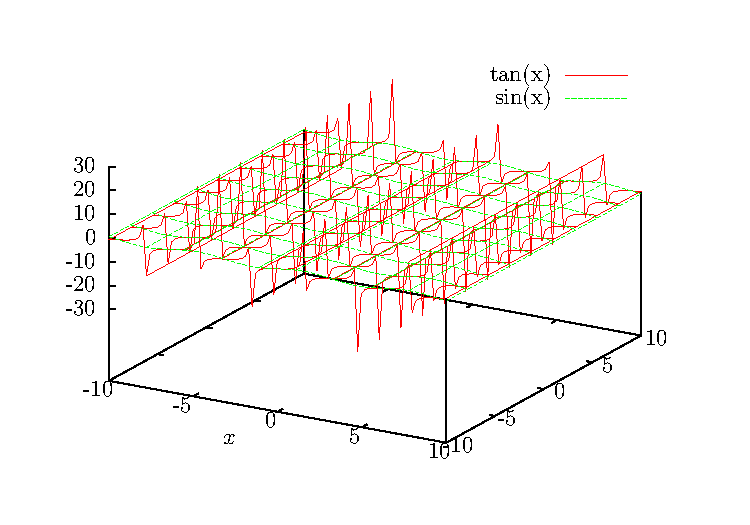
\includegraphics[scale=0.5]{test}
  \end{minipage}}
  \hfill
  \fbox{
  \begin{minipage}[t]{0.4\linewidth}
  	\vspace{0pt}
    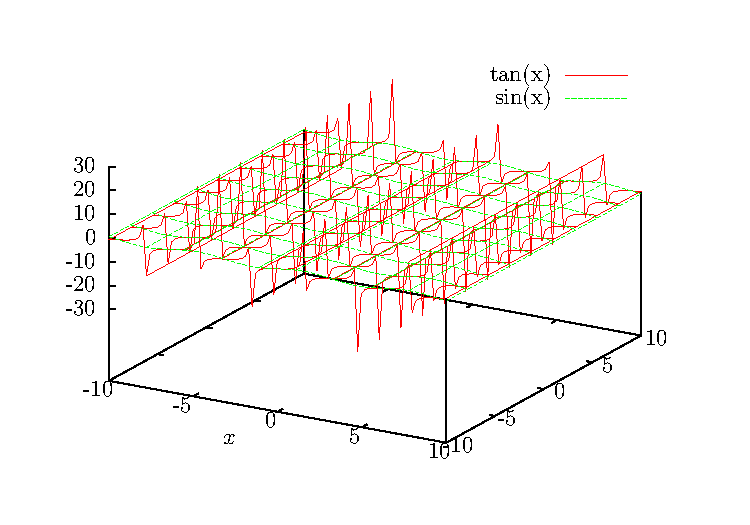
\includegraphics[scale=0.5]{test}
  \end{minipage}
  }
\end{figure}
\blindtext
\begin{longtable}{|ccccp{4cm}|}
\hline
Name & Figure & \# vert. & \# ele. & Description \\
\endfirsthead
Name & Figure & \# vert. & \# ele. & Description \\
\hline
\endhead
\hline
\texttt{square} & 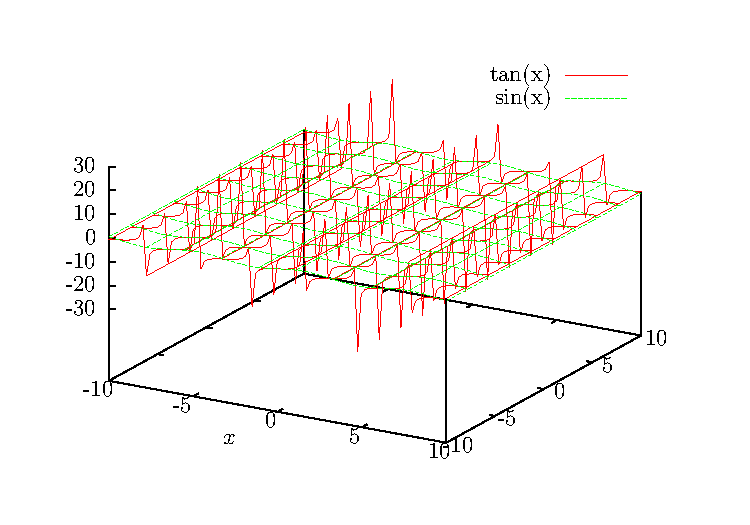
\includegraphics[bb=5cm 9cm 16.5cm 21.5cm, width=4cm]{test} & 7900 & 15613 & TXT1  \\
\hline
\texttt{cube}	&	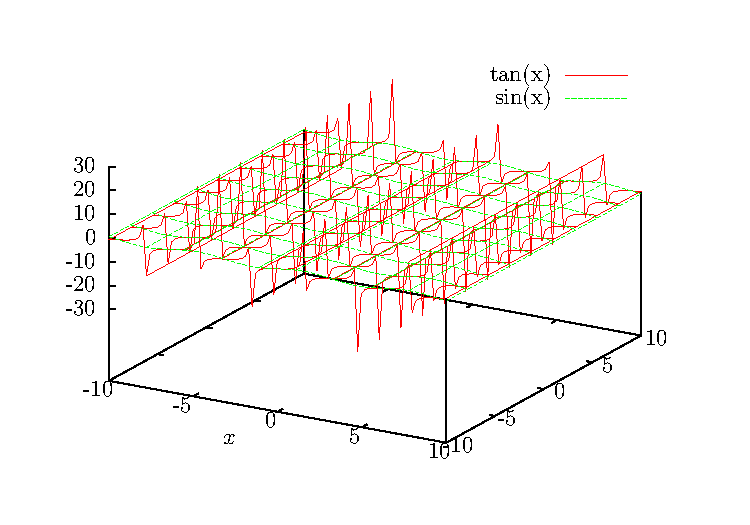
\includegraphics[bb=5cm 9cm 16.5cm 21.5cm, width=4cm]{test} & 3439 & 17727 & TXT2 \\
 
\hline 
 
\end{longtable}
\begin{figure} 
%% LARGER SUBFIGURE 
\subfloat[Caption large box]{% 
\begin{minipage}[c][1\width]{%
 0.5\textwidth} \centering%	
  \includegraphics[width=0.8\textwidth]{box} \end{minipage}} 
  %% SMALLER SUBFIGURE 
  \subfloat[Captopn small box]{% 
  \begin{minipage}[c][1\width]{%
   0.5\textwidth} \centering% 
   \includegraphics[width=0.4\textwidth]{box} \end{minipage}} \caption{Caption of entire figure} \end{figure} 
   
\end{document}